\documentclass[12pt]{article}
\usepackage{fontspec}
\usepackage{xeCJK}
\setCJKmainfont[AutoFakeBold=2]{SimSun}
%\setCJKsansfont{SimHei}
\usepackage{amsmath, amssymb, amsthm}
\usepackage{geometry}
\usepackage{tikz}
\usepackage{fancyhdr}
%\setlength{\headheight}{15pt}
\usetikzlibrary{calc, intersections} % ABX 用於某些符號，若無可刪除
\usepackage{enumitem}
\usepackage{tkz-euclide}
\usepackage{subcaption}
\usepackage{indentfirst}
\usepackage{float}
\usepackage{chngcntr}
\counterwithin{figure}{section}
\counterwithin{figure}{subsection}
\usepackage[most]{tcolorbox}
\usepackage{etoolbox}
% 1. 定義一個新的開關，名字可以自訂（例如：showanswer）
\newtoggle{showanswer}

% 2. 設置開關狀態：true 為開啟（編譯），false 為關閉（不編譯）
\settoggle{showanswer}{true}

\newtcolorbox{mybox}[4][證明]{
  empty,
  breakable,                % 支援跨頁
  sharp corners,
  left=#2+#3,               % 為左側標籤預留空間 (縮進)
  right=0pt, top=0pt, bottom=0pt,
  colback=white,
  % --- 加入以下這行來調整段距 ---
  before upper={\setlength{\parskip}{0.5em plus 0.2em minus 0.1em}},
  after={\vspace{#4}},
  % ---------------------------
  overlay unbroken and first={ % 在第一頁/未斷頁時繪製標籤
    \node[
      anchor=north west,
      draw, 
      inner sep=0pt,
      minimum width=#2,
      minimum height=1.6em, 
      font=\bfseries\boldmath
    ] at (frame.north west) {#1};
  }
}

\geometry{left=1.5cm, right=1.5cm, top=2cm, bottom=2cm}
\counterwithout{figure}{subsection}
% 設定頁首頁尾
\pagestyle{fancy}
\fancyhf{}
\renewcommand{\headrulewidth}{2pt}
\renewcommand{\thefigure}{\thesection-\arabic{figure}} % 主圖編號
\renewcommand{\thesubfigure}{圖 \thesection-\arabic{figure}} % 子圖變為 2-1
\captionsetup[figure]{labelformat=simple, labelsep=quad} 
\captionsetup[subfigure]{labelformat=simple, labelsep=quad} % 移除括號
\renewcommand{\figurename}{圖}
\lhead{廖汶鋒}
\chead{有向角（Directed Angle）}
\rhead{澳門培道中學}
\fancyfoot[C]{\thepage} % Centered footer
%\fancyfoot[L]{2026年2月7日} % Left footer

%\title{四點共圓}
%\author{廖汶鋒}
%\date{2026年2月7日}
\linespread{1.3}

% 定段落首行縮進（兩個中文字）
\setlength{\parindent}{2em}
\setlength{\headheight}{15pt} % 避免頁首高度警告
\begin{document}
\thispagestyle{fancy}  % 讓首頁也顯示頁首
%\maketitle
\begin{center}
    \textbf{\Large{有向角（Directed Angle）}}
\end{center}

\indent 有向角是簡化平面幾何的一個重要利器，它可以透過旋轉方向來進一步精簡許多的幾何定理。
例如平行線判定、四點共圓判定等，都需要考慮幾何圖中的點和線分佈，導致證明時需要分成多種情況討論
但若結合了有向角的知識，所有的情況都能夠歸一化，突出幾何定理的精髓。

本章節主要介紹「直線-直線」和「向量-向量」之間的有向角，給出嚴格定義並建立兩者之間的關係後，重解幾何難題。

\begin{quotation}
    \centering
    \fbox{本內容為原創筆記，未經筆者允許，不得轉發。}
\end{quotation}
\section{直線-直線的有向角}
\subsection{定義}
\begin{mybox}[不嚴格定義1]{7.5em}{1em}{0.5em}
    對於任意兩條直線$l_1$和$l_2$，若$l_1$\ \underline{逆時針}方向旋轉$\theta$角後，能與$l_2$重合或平行，則記
    $$
        \measuredangle{\left(l_1,l_2\right)}=\theta
    $$
    其中，$\theta$稱為$l_1$至$l_2$的有向角。
    \begin{figure}[H]
        \begin{subfigure}[b]{0.45\textwidth}
            \centering
            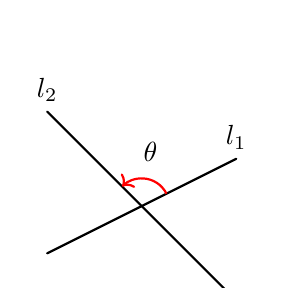
\begin{tikzpicture}[scale=1.2]
                \tkzDefPoints{-1/1/A, 1/-1/C, -1/-0.5/B, 1/0.5/D}
                \tkzInterLL(A,C)(B,D) \tkzGetPoint{O}
                \tkzDrawSegments[black, thick](A,C B,D)
                \tkzPicAngle["$\theta$", draw=red, thick, ->, angle radius=10, angle eccentricity=2](D,O,A)
                \tkzLabelPoint[above](D){$l_1$}
                \tkzLabelPoint[above](A){$l_2$}
            \end{tikzpicture}
            \label{fig:DA_counterclockwise_1_s1}
            \caption{$l_1$逆時針旋轉$\theta$角後，與$l_2$重合（或平行）}
        \end{subfigure}
        \stepcounter{figure}
        \hfill
        \begin{subfigure}[b]{0.45\textwidth}
            \centering
            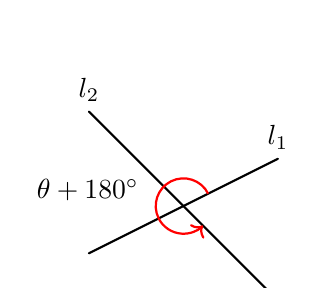
\begin{tikzpicture}[scale=1.2]
                \tkzDefPoints{-1/1/A, 1/-1/C, -1/-0.5/B, 1/0.5/D}
                \tkzInterLL(A,C)(B,D) \tkzGetPoint{O}
                \tkzDrawSegments[black, thick](A,C B,D)
                \tkzPicAngle["$\theta+180^{\circ}$", draw=red, thick, ->, angle radius=10, angle eccentricity=3.5](D,O,C)
                \tkzLabelPoint[above](D){$l_1$}
                \tkzLabelPoint[above](A){$l_2$}
            \end{tikzpicture}
            \label{fig:DA_counterclockwise_2_s1}
            \caption{$l_1$逆時針旋轉$\theta+180^{\circ}$角後，與$l_2$重合（或平行）}
        \end{subfigure}    
    \end{figure}
    如上圖所示，$l_1$分別逆時針旋轉$\theta$、$\theta+180^{\circ}$、$\theta+360^{\circ}$、$\theta+540^{\circ}$、……，
    都能與$l_2$重合或平行，因此有
    $$
        \measuredangle{\left(l_1,l_2\right)}=\theta=\theta+180^{\circ}=\theta+360^{\circ}=\theta+540^{\circ}=\cdots
    $$
\end{mybox}
\newpage
\begin{mybox}[不嚴格定義2]{7.5em}{1em}{0.5em}
    對於任意兩條直線$l_1$和$l_2$，若$l_1$\ \underline{順時針}方向旋轉$\alpha$角後，能與$l_2$重合或平行，則記
    $$
        \measuredangle{\left(l_1,l_2\right)}=-\alpha
    $$
    \begin{figure}[H]
        \begin{subfigure}[b]{0.45\textwidth}
            \centering
            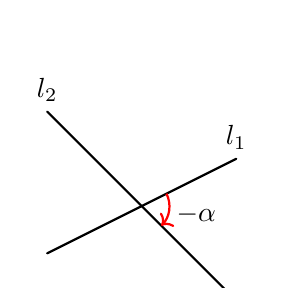
\begin{tikzpicture}[scale=1.2]
                \tkzDefPoints{-1/1/A, 1/-1/C, -1/-0.5/B, 1/0.5/D}
                \tkzInterLL(A,C)(B,D) \tkzGetPoint{O}
                \tkzDrawSegments[black, thick](A,C B,D)
                \tkzPicAngle["$-\alpha$", draw=red, thick, <-, angle radius=10, angle eccentricity=2](C,O,D)
                \tkzLabelPoint[above](D){$l_1$}
                \tkzLabelPoint[above](A){$l_2$}
            \end{tikzpicture}
            \label{fig:DA_clockwise_1_s1}
            \caption{$l_1$順時針旋轉$-\alpha$角後，與$l_2$重合（或平行）}
        \end{subfigure}
        \stepcounter{figure}
        \hfill
        \begin{subfigure}[b]{0.45\textwidth}
            \centering
            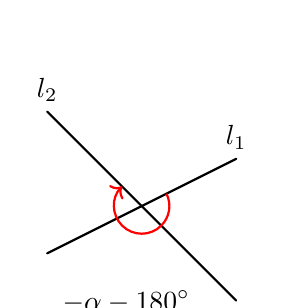
\begin{tikzpicture}[scale=1.2]
                \tkzDefPoints{-1/1/A, 1/-1/C, -1/-0.5/B, 1/0.5/D}
                \tkzInterLL(A,C)(B,D) \tkzGetPoint{O}
                \tkzDrawSegments[black, thick](A,C B,D)
                \tkzPicAngle["$-\alpha-180^{\circ}$", draw=red, thick, <-, angle radius=10, angle eccentricity=3.5](A,O,D)
                \tkzLabelPoint[above](D){$l_1$}
                \tkzLabelPoint[above](A){$l_2$}
            \end{tikzpicture}
            \label{fig:DA_clockwise_2_s1}
            \caption{$l_1$逆時針旋轉$\alpha+180^{\circ}$角後，與$l_2$重合（或平行）}
        \end{subfigure}    
    \end{figure}
    按照此定義，亦容易得知
    $$
        \measuredangle{\left(l_1,l_2\right)}=-\alpha=-\alpha-180^{\circ}=-\alpha-360^{\circ}=-\alpha-540^{\circ}=\cdots
    $$
\end{mybox}
觀察\subref{fig:DA_counterclockwise_1_s1}和\subref{fig:DA_clockwise_1_s1}，
取$\theta\in\left[0^{\circ},180^{\circ}\right)$、$\alpha\in\left(0^{\circ},180^{\circ}\right]$，易知
$$
    \alpha=180^{\circ}-\theta
$$
由此可以導出以下「嚴格定義」。
\begin{mybox}[嚴格定義]{6em}{1em}{0.5em}
    以逆時針旋轉為正方向，順時針旋轉$\alpha$角等價於逆時針旋轉$-\alpha$角。
    若$l_1$\ \underline{逆時針}方向旋轉$\theta$角後，能與$l_2$重合或平行，則記
    $$
        \theta\in\measuredangle{\left(l_1,l_2\right)}
    $$
    其中$\measuredangle{\left(l_1,l_2\right)}$稱為$l_1$至$l_2$所誘導的有向角集合。容易得知$l_1$可以\ \underline{逆時針}方向旋轉……、$\theta-360^{\circ}$、$\theta-180^{\circ}$、
    $\theta$、$\theta+180^{\circ}$、$\theta+360^{\circ}$、……，與$l_2$重合或平行，因此有
    $$
        \measuredangle{\left(l_1,l_2\right)}=\left\{\cdots, \theta-360^{\circ}, \theta-180^{\circ}, \theta, \theta+180^{\circ}, \theta+360^{\circ}, \cdots\right\}=\left\{\theta+180^{\circ}k\left|k\in\mathbb{Z}\right.\right\}
    $$
\end{mybox}
\newpage
\subsection{簡化記號}
\begin{mybox}[三點角]{5em}{1em}{0.5em}
    直線$OA$至直線$OB$的有向角記為
    $$
        \measuredangle{\left(OA,OB\right)}=\measuredangle{AOB}
    $$
    \begin{figure}[H]
        \begin{subfigure}[b]{0.45\textwidth}
            \centering
            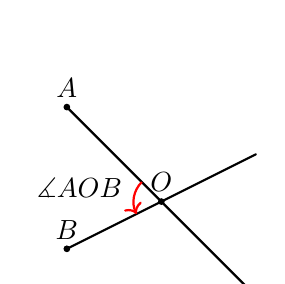
\begin{tikzpicture}[scale=1.2]
                \tkzDefPoints{-1/1/A, 1/-1/C, -1/-0.5/B, 1/0.5/D}
                \tkzInterLL(A,C)(B,D) \tkzGetPoint{O}
                \tkzDrawSegments[black, thick](A,C B,D)
                \tkzPicAngle["$\measuredangle{AOB}$", draw=red, thick, ->, angle radius=10, angle eccentricity=3](A,O,B)
                \tkzDrawPoints[fill=black](A,B,O)
                \tkzLabelPoints[above](A,B,O)
            \end{tikzpicture}
            \label{fig:DA_s1-3}
            \caption{$OA$逆時針旋轉一個劣角後，與$OB$重合（或平行）}
        \end{subfigure}
        \stepcounter{figure}
        \hfill
        \begin{subfigure}[b]{0.45\textwidth}
            \centering
            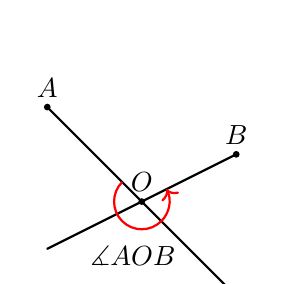
\begin{tikzpicture}[scale=1.2]
                \tkzDefPoints{-1/1/A, 1/-1/C, -1/-0.5/D, 1/0.5/B}
                \tkzInterLL(A,C)(B,D) \tkzGetPoint{O}
                \tkzDrawSegments[black, thick](A,C B,D)
                \tkzPicAngle["$\measuredangle{AOB}$", draw=red, thick, ->, angle radius=10, angle eccentricity=2](A,O,B)
                \tkzDrawPoints[fill=black](A,B,O)
                \tkzLabelPoints[above](A,B,O)
            \end{tikzpicture}
            \label{fig:DA_s1-4}
            \caption{$OA$逆時針旋轉一個優角後，與$OB$重合（或平行）}
        \end{subfigure}    
    \end{figure}
\end{mybox}
\begin{mybox}[集合-角度]{6em}{1em}{0.5em}
    因為$\measuredangle{\left(l_1,l_2\right)}$是一個集合，而$\theta$只是集合中的一個元素，
    為了避免每次在利用有向角時都要引入「$\forall \theta\in\measuredangle{\left(l_1,l_2\right)}$」這種繁瑣寫法，
    所以引入以下兩種等價寫法：
    \begin{enumerate}
        \item $\measuredangle{\left(l_1,l_2\right)}=\theta$
        \item $\measuredangle{\left(l_1,l_2\right)}\equiv\theta\quad\left(\text{mod}\ {180^{\circ}}\right)$
        \item $\measuredangle{\left(l_1,l_2\right)}\equiv\theta\quad\left(\text{mod}\ {\pi}\right)$
    \end{enumerate}
\end{mybox}
\subsection{運算}
\begin{mybox}[集合-集合加法]{8.5em}{1em}{0.5em}
    對於任意四條直線$l_1$、$l_2$、$l_3$和$l_4$，
    設$\measuredangle{\left(l_1,l_2\right)}=\alpha$、$\measuredangle{\left(l_3,l_4\right)}=\beta$，定義
    $$
        \measuredangle{\left(l_1,l_2\right)}\pm\measuredangle{\left(l_3,l_4\right)}=\left\{\alpha\pm\beta+180^{\circ}k\left|k\in\mathbb{Z}\right.\right\}
    $$
    注意，這裏的「加法」是定義在集合$\measuredangle{\left(l_1,l_2\right)}$和$\measuredangle{\left(l_3,l_4\right)}$之間的。
    
    採用簡化記號後可得以下三式：
    \begin{enumerate}
        \item $\measuredangle{\left(l_1,l_2\right)}\pm\measuredangle{\left(l_3,l_4\right)}=\alpha\pm\beta$
        \item $\measuredangle{\left(l_1,l_2\right)}\pm\measuredangle{\left(l_3,l_4\right)}\equiv\alpha\pm\beta\left(\text{mod}\ {180^{\circ}}\right)$
        \item $\measuredangle{\left(l_1,l_2\right)}\pm\measuredangle{\left(l_3,l_4\right)}\equiv\alpha\pm\beta\left(\text{mod}\ {\pi}\right)$
    \end{enumerate}
    這裏可以體現，簡化記號能把集合之間的加法直接轉換成元素之間的加法。
\end{mybox}
\begin{mybox}[集合-角度值加法]{9.5em}{1em}{0.5em}
    對於任意兩條直線$l_1$和$l_2$，以及任意角度值$\varphi$。
    設$\measuredangle{\left(l_1,l_2\right)}=\theta$，定義
    $$
        \measuredangle{\left(l_1,l_2\right)}\pm\varphi=\left\{\theta\pm\varphi+180^{\circ}k\left|k\in\mathbb{Z}\right.\right\}
    $$
    注意，這裏的「加法」是定義在集合$\measuredangle{\left(l_1,l_2\right)}$和角度值$\varphi$之間的。
    
    採用簡化記號後可得以下三式：
    \begin{enumerate}
        \item $\measuredangle{\left(l_1,l_2\right)}\pm\varphi=\theta\pm\varphi$
        \item $\measuredangle{\left(l_1,l_2\right)}\pm\varphi\equiv\theta\pm\varphi\left(\text{mod}\ {180^{\circ}}\right)$
        \item $\measuredangle{\left(l_1,l_2\right)}\pm\varphi\equiv\theta\pm\varphi\left(\text{mod}\ {\pi}\right)$
    \end{enumerate}
    這裏可以體現，簡化記號能把集合與角度值之間的加法直接轉換成數值之間的加法。
\end{mybox}
\begin{mybox}[乘法]{4em}{1em}{0.5em}
    對於任意兩條直線$l_1$和$l_2$，以及任意實數$\beta\in\mathbb{R}$，若$\measuredangle{\left(l_1,l_2\right)}=\theta$，定義
    $$
        \beta\measuredangle{\left(l_1,l_2\right)}=\left\{\beta\left(\theta+180^{\circ}k\right)\left|k\in\mathbb{Z}\right.\right\}
    $$
    此時第一種簡化記號失效（盡量不要使用，否則會引起歧義）

    當$\beta\neq0$時，才可以採用第二或三種簡化記號：
    \begin{enumerate}[start=2]
        \item $\beta\measuredangle{\left(l_1,l_2\right)}\equiv\beta\theta\left(\text{mod}\ {180^{\circ}|\beta|}\right)$
        \item $\beta\measuredangle{\left(l_1,l_2\right)}\equiv\beta\theta\left(\text{mod}\ {|\beta|\pi}\right)$
    \end{enumerate}
\end{mybox}
\subsection{性質}
基於有向角的運算，結合實際幾何知識，可以推出以下性質：
\begin{mybox}[性質1]{4.5em}{1em}{0.5em}
    對於任意三條直線$l_1$、$l_2$和$l_3$，都有
    $$
        \measuredangle{\left(l_1,l_2\right)}+\measuredangle{\left(l_2,l_3\right)}=\measuredangle{\left(l_1,l_3\right)}
    $$
    這表明$l_1$先旋轉至與$l_2$平行（或重合），再旋轉至與$l_3$平行（或重合）的效果，和$l_1$直接旋轉至與$l_3$平行（或重合）的效果是一致的。
\end{mybox}
\begin{mybox}[性質2]{4.5em}{1em}{0.5em}
    對於任意直線$l$都有
    $$
        \measuredangle{\left(l,l\right)}=0^{\circ}
    $$
    此性質可由性質1推導得。（取$l_1=l_2=l_3=l$）
\end{mybox}
\begin{mybox}[性質3]{4.5em}{1em}{0.5em}
    對於任意兩條直線$l_1$和$l_2$，都有
    $$
        \measuredangle{\left(l_1,l_2\right)}=-\measuredangle{\left(l_2,l_1\right)}
    $$
    此性質可由性質1和2推導得。（取$l_3=l_1$）

    此性質說明了$l_1$逆時針旋轉$\theta$後與$l_2$平行（或重合），等價於$l_2$順時針旋轉$\theta$後與$l_1$平行（或重合）。
\end{mybox}

以上三個性質可以與向量的性質作類比，如下表所示：
\begin{table}[H]
    \centering
    \begin{tabular}{|c|c|c|}
        \hline
        &向量&有向角\\
        \hline
        加法性&$\overrightarrow{AB}+\overrightarrow{BC}=\overrightarrow{AC}$
        &$\measuredangle{\left(l_1,l_2\right)}+\measuredangle{\left(l_2,l_3\right)}=\measuredangle{\left(l_1,l_3\right)}$\\
        \hline
        零元&$\overrightarrow{AA}=\overrightarrow{0}$&$\measuredangle{\left(l,l\right)}=0^{\circ}$\\
        \hline
        負交換律&$\overrightarrow{AB}=-\overrightarrow{BA}$&$\measuredangle{\left(l_1,l_2\right)}=-\measuredangle{\left(l_2,l_1\right)}$\\
        \hline
    \end{tabular}
\end{table}
\begin{mybox}[性質4]{4.5em}{1em}{0.5em}
    對於兩條垂直線$l_1$和$l_2$，都有
    $$
        \measuredangle{\left(l_1,l_2\right)}=90^{\circ}
    $$
\end{mybox}
\subsection{禁忌}
\begin{mybox}[禁忌1]{4.5em}{1em}{0.5em}
    對於$\beta\measuredangle{\left(l_1,l_2\right)}$，當$\beta\notin\mathbb{Z}$時，不能把$\beta\measuredangle{\left(l_1,l_2\right)}$代入至任一個三角函數中使用。
\end{mybox}
\begin{mybox}[禁忌2]{4.5em}{1em}{0.5em}
    對於$\beta\measuredangle{\left(l_1,l_2\right)}$，當$\beta$不為偶數時，不能把$\beta\measuredangle{\left(l_1,l_2\right)}$代入至$\sin{}$、$\cos{}$、$\csc{}$或$\sec{}$函數中使用。
\end{mybox}
\begin{mybox}[禁忌3]{4.5em}{1em}{0.5em}
    對於$\beta\measuredangle{\left(l_1,l_2\right)}$，當$\beta\in\mathbb{Z}^+\setminus\left\{1\right\}$時，以下不等式嚴格成立
    $$
        \beta\measuredangle{\left(l_1,l_2\right)}\neq\sum\limits_{i=1}^{\beta}{\measuredangle{\left(l_1,l_2\right)}}
    $$
\end{mybox}
\subsection{允許}
此章節亦屬於《有向角的性質》，但為了照顧初次接觸有向角的讀者，所以筆者將此部分內容單獨整理成一個章節。

另一方面，此章節與上一節是一一對應的，請讀者自行領悟：
\begin{mybox}[允許1]{4.5em}{1em}{0.5em}
    對於$\beta\measuredangle{\left(l_1,l_2\right)}$，當$\beta$是整數時，
    $\tan{\left[\beta\measuredangle{\left(l_1,l_2\right)}\right]}$的取值是唯一的。
\end{mybox}
\begin{mybox}[證明]{4em}{1em}{0.5em}
    當$\beta=0$時，$\beta\measuredangle{\left(l_1,l_2\right)}=\left\{0^{\circ}\right\}$，所以$\tan{\left[\beta\measuredangle{\left(l_1,l_2\right)}\right]}=0$。

    當$\beta\in\mathbb{Z}\setminus\left\{0\right\}$時，$\forall \theta_1,\theta_2\in\beta\measuredangle{\left(l_1,l_2\right)}$，由乘法的定義可得
    $$
        \theta_1\equiv\theta_2\left(\text{mod}\ {180^{\circ}|\beta|}\right)
    $$
    因為$\beta$是非零整數，所以由同餘的性質可知
    $$
        \theta_1\equiv\theta_2\left(\text{mod}\ {180^{\circ}}\right)
    $$
    結合$\tan$函數的最小正周期可知
    $$
        \tan{\theta_1}=\tan{\theta_2}
    $$
    即$\tan{\measuredangle{\left(l_1,l_2\right)}}$的取值是唯一的。
\end{mybox}
\begin{mybox}[允許2]{4.5em}{1em}{0.5em}
    對於$\beta\measuredangle{\left(l_1,l_2\right)}$，當$\beta$是偶數時，
    $\sin{\left[\beta\measuredangle{\left(l_1,l_2\right)}\right]}$和$\cos{\left[\beta\measuredangle{\left(l_1,l_2\right)}\right]}$的取值是唯一的。
\end{mybox}
\begin{mybox}[證明]{4em}{1em}{0.5em}
    當$\beta=0$時，$\beta\measuredangle{\left(l_1,l_2\right)}=\left\{0^{\circ}\right\}$，
    所以$\sin{\left[\beta\measuredangle{\left(l_1,l_2\right)}\right]}=0$和$\cos{\left[\beta\measuredangle{\left(l_1,l_2\right)}\right]}=1$。

    當$\beta$是非零偶數時，$\forall \theta_1,\theta_2\in\beta\measuredangle{\left(l_1,l_2\right)}$，由乘法的定義可得
    $$
        \theta_1\equiv\theta_2\left(\text{mod}\ {180^{\circ}|\beta|}\right)
    $$
    因為$\beta$是非零偶數，所以由同餘的性質可知
    $$
        \theta_1\equiv\theta_2\left(\text{mod}\ {360^{\circ}}\right)
    $$
    結合$\sin{}$和$\cos{}$函數的最小正周期可知
    $$
        \sin{\theta_1}=\sin{\theta_2},\quad \cos{\theta_1}=\cos{\theta_2}
    $$
    即$\sin{\left[\beta\measuredangle{\left(l_1,l_2\right)}\right]}$和$\cos{\left[\beta\measuredangle{\left(l_1,l_2\right)}\right]}$的取值是唯一的。
\end{mybox}
\begin{mybox}[允許3]{4.5em}{1em}{0.5em}
    對於$\beta\measuredangle{\left(l_1,l_2\right)}$，當$\beta\in\mathbb{N}$時，以下不等式成立
    $$
        \beta\measuredangle{\left(l_1,l_2\right)}\subseteq\sum\limits_{i=1}^{\beta}{\measuredangle{\left(l_1,l_2\right)}}
    $$
    等號成立當且僅當$\beta=1$。
\end{mybox}
\begin{mybox}[證明]{4em}{1em}{0.5em}
    當$\beta=0$時，$\beta\measuredangle{\left(l_1,l_2\right)}=\left\{0\right\}$，$\sum\limits_{i=1}^{\beta}{\measuredangle{\left(l_1,l_2\right)}}=\left\{180^{\circ}k\left|k\in\mathbb{Z}\right.\right\}$。
    
    當$\beta=1$時，$\beta\measuredangle{\left(l_1,l_2\right)}=\measuredangle{\left(l_1,l_2\right)}=\sum\limits_{i=1}^{\beta}{\measuredangle{\left(l_1,l_2\right)}}$。

    當$\beta\in\mathbb{N}\setminus\left\{0,1\right\}$時，設$\measuredangle{\left(l_1,l_2\right)}=\theta$，
    則對於$\beta\measuredangle{\left(l_1,l_2\right)}$的任一元素$\varphi$都有
    $$
        \varphi\equiv\beta\theta\quad\left(\text{mod}\ {180^{\circ}\beta}\right)
    $$
    因為$\beta$是非零整數，所以由同餘的性質可知
    $$
        \varphi\equiv\beta\theta\quad\left(\text{mod}\ {180^{\circ}}\right)
    $$
    所以有$\varphi\in\sum\limits_{i=1}^{\beta}{\measuredangle{\left(l_1,l_2\right)}}$，即有
    $$
        \beta\measuredangle{\left(l_1,l_2\right)}\subseteq\sum\limits_{i=1}^{\beta}{\measuredangle{\left(l_1,l_2\right)}}
    $$
    另一方面，取$\sum\limits_{i=1}^{\beta}{\measuredangle{\left(l_1,l_2\right)}}$的其中一個元素$\beta\theta+180^{\circ}$。
    \begin{align*}
        \beta\theta+180^{\circ}-\beta\measuredangle{\left(l_1,l_2\right)}&\equiv180^{\circ}\quad\left(\text{mod}\ {180^{\circ}\beta}\right)\\
        &\neq0^{\circ}\quad\left(\text{mod}\ {180^{\circ}\beta}\right)
    \end{align*}
    即$\beta\theta+180^{\circ}\notin\beta\measuredangle{\left(l_1,l_2\right)}$，所以當$\beta\in\mathbb{N}\setminus\left\{1\right\}$時
    $$
        \beta\measuredangle{\left(l_1,l_2\right)}\subsetneqq\sum\limits_{i=1}^{\beta}{\measuredangle{\left(l_1,l_2\right)}}
    $$
\end{mybox}
\newpage
\section{向量-向量的有向角}
\subsection{定義}
參考《直線-直線的有向角》，可以得出以下「嚴格定義」。
\begin{mybox}[嚴格定義]{6em}{1em}{0.5em}
    以逆時針旋轉為正方向，順時針旋轉$\alpha$角等價於逆時針旋轉$-\alpha$角。
    若非零向量$\overrightarrow{AC}$\ \underline{逆時針}方向旋轉$\theta$角後，能與非零向量$\overrightarrow{BD}$同向平行，則記
    $$
        \theta\in\measuredangle{\left(\overrightarrow{AC},\overrightarrow{BD}\right)}
    $$
    \begin{figure}[H]
        \begin{subfigure}[b]{0.45\textwidth}
            \centering
            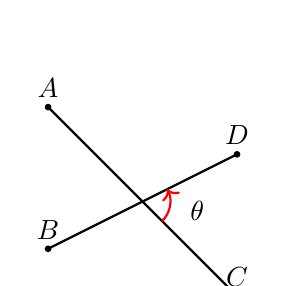
\begin{tikzpicture}[scale=1.2]
                \tkzDefPoints{-1/1/A, 1/-1/C, -1/-0.5/B, 1/0.5/D}
                \tkzInterLL(A,C)(B,D) \tkzGetPoint{O}
                \tkzDrawSegments[black, thick](A,C B,D)
                \tkzPicAngle["$\theta$", draw=red, thick, ->, angle radius=10, angle eccentricity=2](C,O,D)
                \tkzDrawPoints[fill=black](A,B,C,D)
                \tkzLabelPoints[above](A,B,C,D)
            \end{tikzpicture}
            \label{fig:DA_counterclockwise_1_s2}
            \caption{$\overrightarrow{OA}$逆時針旋轉$\theta$後，與$\overrightarrow{OB}$重合（或平行）}
        \end{subfigure}
        \stepcounter{figure}
        \hfill
        \begin{subfigure}[b]{0.45\textwidth}
            \centering
            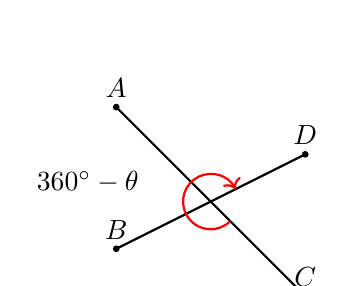
\begin{tikzpicture}[scale=1.2]
                \tkzDefPoints{-1/1/A, 1/-1/C, -1/-0.5/B, 1/0.5/D}
                \tkzInterLL(A,C)(B,D) \tkzGetPoint{O}
                \tkzDrawSegments[black, thick](A,C B,D)
                \tkzPicAngle["$360^{\circ}-\theta$", draw=red, thick, <-, angle radius=10, angle eccentricity=4.5](D,O,C)
                \tkzDrawPoints[fill=black](A,B,C,D)
                \tkzLabelPoints[above](A,B,C,D)
            \end{tikzpicture}
            \label{fig:DA_clockwise_1_s2}
            \caption{$\overrightarrow{OA}$順時針旋轉$360^{\circ}-\theta$後，與$\overrightarrow{OB}$重合（或平行）}
        \end{subfigure}    
    \end{figure}
    
    其中$\measuredangle{\left(\overrightarrow{AC},\overrightarrow{BD}\right)}$稱為$\overrightarrow{AC}$至$\overrightarrow{BD}$所誘導的有向角集合。
    容易得知$\overrightarrow{AC}$可以\ \underline{逆時針}方向旋轉……、$\theta-720^{\circ}$、$\theta-360^{\circ}$、
    $\theta$、$\theta+360^{\circ}$、$\theta+720^{\circ}$、……，與$\overrightarrow{BD}$同向平行，因此有
    $$
        \measuredangle{\left(\overrightarrow{AC},\overrightarrow{BD}\right)}
        =\left\{\cdots, \theta-720^{\circ}, \theta-360^{\circ}, \theta, \theta+360^{\circ}, \theta+720^{\circ}, \cdots\right\}
        =\left\{\theta+360^{\circ}k\left|k\in\mathbb{Z}\right.\right\}
    $$
\end{mybox}
\subsection{簡化記號}
\begin{mybox}[三點角]{5em}{1em}{0.5em}
    向量非零向量$\overrightarrow{OA}$至$\overrightarrow{OB}$的有向角記為
    $$
        \measuredangle{\left(\overrightarrow{OA},\overrightarrow{OB}\right)}=\measuredangle{\overrightarrow{AOB}}
    $$
    \begin{figure}[H]
        \begin{subfigure}[b]{0.45\textwidth}
            \centering
            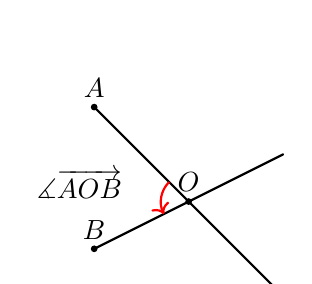
\begin{tikzpicture}[scale=1.2]
                \tkzDefPoints{-1/1/A, 1/-1/C, -1/-0.5/B, 1/0.5/D}
                \tkzInterLL(A,C)(B,D) \tkzGetPoint{O}
                \tkzDrawSegments[black, thick](A,C B,D)
                \tkzPicAngle["$\measuredangle{\overrightarrow{AOB}}$", draw=red, thick, ->, angle radius=10, angle eccentricity=4](A,O,B)
                \tkzDrawPoints[fill=black](A,B,O)
                \tkzLabelPoints[above](A,B,O)
            \end{tikzpicture}
            \label{fig:DA_s2-3}
            \caption{$\overrightarrow{OA}$逆時針旋轉一個劣角後，與$\overrightarrow{OB}$重合（或平行）}
        \end{subfigure}
        \stepcounter{figure}
        \hfill
        \begin{subfigure}[b]{0.45\textwidth}
            \centering
            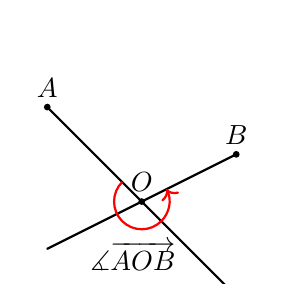
\begin{tikzpicture}[scale=1.2]
                \tkzDefPoints{-1/1/A, 1/-1/C, -1/-0.5/D, 1/0.5/B}
                \tkzInterLL(A,C)(B,D) \tkzGetPoint{O}
                \tkzDrawSegments[black, thick](A,C B,D)
                \tkzPicAngle["$\measuredangle{\overrightarrow{AOB}}$", draw=red, thick, ->, angle radius=10, angle eccentricity=2](A,O,B)
                \tkzDrawPoints[fill=black](A,B,O)
                \tkzLabelPoints[above](A,B,O)
            \end{tikzpicture}
            \label{fig:DA_s2-4}
            \caption{$\overrightarrow{OA}$逆時針旋轉一個優角後，與$\overrightarrow{OB}$重合（或平行）}
        \end{subfigure}    
    \end{figure}
\end{mybox}
\begin{mybox}[集合-角度]{6em}{1em}{0.5em}
    對於任意非零向量$\overrightarrow{v_1}$和$\overrightarrow{v_2}$，$\measuredangle{\left(\overrightarrow{v_1},\overrightarrow{v_2}\right)}$是一個集合，
    而$\theta$只是集合中的一個元素，為了避免每次在利用有向角時都要引入「$\forall \theta\in\measuredangle{\left(\overrightarrow{v_1},\overrightarrow{v_2}\right)}$」這種繁瑣寫法，
    所以引入以下兩種等價寫法：
    \begin{enumerate}
        \item $\measuredangle{\left(\overrightarrow{v_1},\overrightarrow{v_2}\right)}=\theta$
        \item $\measuredangle{\left(\overrightarrow{v_1},\overrightarrow{v_2}\right)}\equiv\theta\quad\left(\text{mod}\ {360^{\circ}}\right)$
        \item $\measuredangle{\left(\overrightarrow{v_1},\overrightarrow{v_2}\right)}\equiv\theta\quad\left(\text{mod}\ {2\pi}\right)$
    \end{enumerate}
\end{mybox}
\subsection{運算}
\begin{mybox}[集合-集合加法]{8.5em}{1em}{0.5em}
    對於任意四個非零向量$\overrightarrow{v_1}$、$\overrightarrow{v_2}$、$\overrightarrow{v_3}$和$\overrightarrow{v_4}$，
    設$\measuredangle{\left(\overrightarrow{v_1},\overrightarrow{v_2}\right)}=\alpha$、$\measuredangle{\left(\overrightarrow{v_3},\overrightarrow{v_4}\right)}=\beta$，定義
    $$
        \measuredangle{\left(\overrightarrow{v_1},\overrightarrow{v_2}\right)}\pm\measuredangle{\left(\overrightarrow{v_3},\overrightarrow{v_4}\right)}
        =\left\{\alpha\pm\beta+180^{\circ}k\left|k\in\mathbb{Z}\right.\right\}
    $$
    注意，這裏的「加法」是定義在集合$\measuredangle{\left(\overrightarrow{v_1},\overrightarrow{v_2}\right)}$和$\measuredangle{\left(\overrightarrow{v_3},\overrightarrow{v_4}\right)}$之間的。
    
    採用簡化記號後可得以下三式：
    \begin{enumerate}
        \item $\measuredangle{\left(\overrightarrow{v_1},\overrightarrow{v_2}\right)}\pm\measuredangle{\left(\overrightarrow{v_3},\overrightarrow{v_4}\right)}=\alpha\pm\beta$
        \item $\measuredangle{\left(\overrightarrow{v_1},\overrightarrow{v_2}\right)}\pm\measuredangle{\left(\overrightarrow{v_3},\overrightarrow{v_4}\right)}\equiv\alpha\pm\beta\quad\left(\text{mod}\ {360^{\circ}}\right)$
        \item $\measuredangle{\left(\overrightarrow{v_1},\overrightarrow{v_2}\right)}\pm\measuredangle{\left(\overrightarrow{v_3},\overrightarrow{v_4}\right)}\equiv\alpha\pm\beta\quad\left(\text{mod}\ {2\pi}\right)$
    \end{enumerate}
    這裏可以體現，簡化記號能把集合之間的加法直接轉換成元素之間的加法。
\end{mybox}
\begin{mybox}[集合-角度值加法]{9.5em}{1em}{0.5em}
    對於任意兩個非零向量$\overrightarrow{v_1}$和$\overrightarrow{v_2}$，以及任意角度值$\varphi$。
    設$\measuredangle{\left(\overrightarrow{v_1},\overrightarrow{v_2}\right)}=\theta$，定義
    $$
        \measuredangle{\left(\overrightarrow{v_1},\overrightarrow{v_2}\right)}\pm\varphi=\left\{\theta\pm\varphi+360^{\circ}k\left|k\in\mathbb{Z}\right.\right\}
    $$
    注意，這裏的「加法」是定義在集合$\measuredangle{\left(l_1,l_2\right)}$和角度值$\varphi$之間的。
    
    採用簡化記號後可得以下三式：
    \begin{enumerate}
        \item $\measuredangle{\left(\overrightarrow{v_1},\overrightarrow{v_2}\right)}\pm\varphi=\theta\pm\varphi$
        \item $\measuredangle{\left(\overrightarrow{v_1},\overrightarrow{v_2}\right)}\pm\varphi\equiv\theta\pm\varphi\quad\left(\text{mod}\ {360^{\circ}}\right)$
        \item $\measuredangle{\left(\overrightarrow{v_1},\overrightarrow{v_2}\right)}\pm\varphi\equiv\theta\pm\varphi\quad\left(\text{mod}\ {2\pi}\right)$
    \end{enumerate}
    這裏可以體現，簡化記號能把集合與角度值之間的加法直接轉換成數值之間的加法。
\end{mybox}
\begin{mybox}[乘法]{4em}{1em}{0.5em}
    對於任意兩個非零向量$\overrightarrow{v_1}$和$\overrightarrow{v_2}$，以及任意實數$\beta\in\mathbb{R}$，
    若$\measuredangle{\left(\overrightarrow{v_1},\overrightarrow{v_2}\right)}=\theta$，定義
    $$
        \beta\measuredangle{\left(\overrightarrow{v_1},\overrightarrow{v_2}\right)}=\left\{\beta\left(\theta+360^{\circ}k\right)\left|k\in\mathbb{Z}\right.\right\}
    $$
    此時第一種簡化記號失效（盡量不要使用，否則會引起歧義）

    當$\beta\neq0$時，才可以採用第二或三種簡化記號：
    \begin{enumerate}[start=2]
        \item $\beta\measuredangle{\left(\overrightarrow{v_1},\overrightarrow{v_2}\right)}\equiv\beta\theta\quad\left(\text{mod}\ {360^{\circ}|\beta|}\right)$
        \item $\beta\measuredangle{\left(\overrightarrow{v_1},\overrightarrow{v_2}\right)}\equiv\beta\theta\quad\left(\text{mod}\ {2|\beta|\pi}\right)$
    \end{enumerate}
\end{mybox}
\subsection{性質}
基於有向角的運算，結合實際幾何知識，可以推出以下性質：
\begin{mybox}[性質1]{4.5em}{1em}{0.5em}
    對於任意三個非零向量$\overrightarrow{v_1}$、$\overrightarrow{v_2}$和$\overrightarrow{v_3}$，都有
    $$
        \measuredangle{\left(\overrightarrow{v_1},\overrightarrow{v_2}\right)}+\measuredangle{\left(\overrightarrow{v_2},\overrightarrow{v_3}\right)}
        =\measuredangle{\left(\overrightarrow{v_1},\overrightarrow{v_3}\right)}
    $$
    這表明$\overrightarrow{v_1}$先旋轉至與$\overrightarrow{v_2}$同向平行，
    再旋轉至與$\overrightarrow{v_3}$同向平行（或重合）的效果，和$\overrightarrow{v_1}$直接旋轉至與$\overrightarrow{v_3}$同向平行的效果是一致的。
\end{mybox}
\begin{mybox}[性質2]{4.5em}{1em}{0.5em}
    對於任意非零向量$\overrightarrow{v}$都有
    $$
        \measuredangle{\left(\overrightarrow{v},\overrightarrow{v}\right)}=0^{\circ}
    $$
    此性質可由性質1推導得。（取$\overrightarrow{v_1}=\overrightarrow{v_2}=\overrightarrow{v_3}=\overrightarrow{v}$）
\end{mybox}
\begin{mybox}[性質3]{4.5em}{1em}{0.5em}
    對於任意兩個非零向量$\overrightarrow{v_1}$和$\overrightarrow{v_2}$，都有
    $$
        \measuredangle{\left(\overrightarrow{v_1},\overrightarrow{v_2}\right)}=-\measuredangle{\left(\overrightarrow{v_2},\overrightarrow{v_1}\right)}
    $$
    此性質可由性質1和2推導得。（取$\overrightarrow{v_3}=\overrightarrow{v_1}$）

    此性質說明了$\overrightarrow{v_1}$逆時針旋轉$\theta$後與$\overrightarrow{v_2}$同向平行，等價於$\overrightarrow{v_2}$順時針旋轉$\theta$後與$\overrightarrow{v_1}$同向平行。
\end{mybox}

以上所有性質可以與向量的性質作類比，如下表所示：
\begin{table}[H]
    \centering
    \begin{tabular}{|c|c|c|c|}
        \hline
        &向量&直線有向角&向量有向角\\
        \hline
        加法性&$\overrightarrow{AB}+\overrightarrow{BC}=\overrightarrow{AC}$
        &$\measuredangle{\left(l_1,l_2\right)}+\measuredangle{\left(l_2,l_3\right)}=\measuredangle{\left(l_1,l_3\right)}$
        &$\measuredangle{\left(\overrightarrow{v_1},\overrightarrow{v_2}\right)}+\measuredangle{\left(\overrightarrow{v_2},\overrightarrow{v_3}\right)}
        =\measuredangle{\left(\overrightarrow{v_1},\overrightarrow{v_3}\right)}$\\
        \hline
        零元&$\overrightarrow{AA}=\overrightarrow{0}$&$\measuredangle{\left(l,l\right)}=0^{\circ}$
        &$\measuredangle{\left(\overrightarrow{v},\overrightarrow{v}\right)}=0^{\circ}$\\
        \hline
        負交換律&$\overrightarrow{AB}=-\overrightarrow{BA}$&$\measuredangle{\left(l_1,l_2\right)}=-\measuredangle{\left(l_2,l_1\right)}$
        &$\measuredangle{\left(\overrightarrow{v_1},\overrightarrow{v_2}\right)}=-\measuredangle{\left(\overrightarrow{v_2},\overrightarrow{v_1}\right)}$\\
        \hline
    \end{tabular}
\end{table}
\begin{mybox}[性質4]{4.5em}{1em}{0.5em}
    對於任意非零向量$\overrightarrow{v}$都有
    $$
        \measuredangle{\left(\overrightarrow{v},-\overrightarrow{v}\right)}=180^{\circ}
    $$
\end{mybox}
\begin{mybox}[性質5]{4.5em}{1em}{0.5em}
    對於任意兩個非零向量$\overrightarrow{v_1}$和$\overrightarrow{v_2}$，都有
    $$
        \measuredangle{\left(\overrightarrow{v_1},-\overrightarrow{v_2}\right)}
        =\measuredangle{\left(-\overrightarrow{v_1},\overrightarrow{v_2}\right)}
        =\measuredangle{\left(\overrightarrow{v_1},\overrightarrow{v_2}\right)}+180^{\circ}
    $$
    此性質可由性質1和4推導得。
\end{mybox}
\begin{mybox}[性質6]{4.5em}{1em}{0.5em}
    對於任意兩個非零向量$\overrightarrow{v_1}$和$\overrightarrow{v_2}$，都有
    $$
        \measuredangle{\left(-\overrightarrow{v_1},-\overrightarrow{v_2}\right)}
        =\measuredangle{\left(\overrightarrow{v_1},\overrightarrow{v_2}\right)}
    $$
\end{mybox}
\subsection{禁忌}
\begin{mybox}[禁忌1]{4.5em}{1em}{0.5em}
    對於$\beta\measuredangle{\left(\overrightarrow{v_1},\overrightarrow{v_2}\right)}$，
    當$2\beta\notin\mathbb{Z}$時，不能把$\beta\measuredangle{\left(\overrightarrow{v_1},\overrightarrow{v_2}\right)}$代入至任一個三角函數中使用。
\end{mybox}
\begin{mybox}[禁忌2]{4.5em}{1em}{0.5em}
    對於$\beta\measuredangle{\left(\overrightarrow{v_1},\overrightarrow{v_2}\right)}$，
    當$\beta$不為整數時，不能把$\beta\measuredangle{\left(\overrightarrow{v_1},\overrightarrow{v_2}\right)}$代入至$\sin{}$、$\cos{}$、$\csc{}$或$\sec{}$函數中使用。
\end{mybox}
\begin{mybox}[禁忌3]{4.5em}{1em}{0.5em}
    對於$\beta\measuredangle{\left(\overrightarrow{v_1},\overrightarrow{v_2}\right)}$，當$\beta\in\mathbb{Z}^+\setminus\left\{1\right\}$時，以下不等式嚴格成立
    $$
        \beta\measuredangle{\left(\overrightarrow{v_1},\overrightarrow{v_2}\right)}
        \neq\sum\limits_{i=1}^{\beta}{\measuredangle{\left(\overrightarrow{v_1},\overrightarrow{v_2}\right)}}
    $$
\end{mybox}
\subsection{允許}
此章節亦屬於《有向角的性質》，但為了照顧初次接觸有向角的讀者，所以筆者將此部分內容單獨整理成一個章節。

另一方面，此章節與上一節是一一對應的，請讀者自行領悟：
\begin{mybox}[允許1]{4.5em}{1em}{0.5em}
    對於$\beta\measuredangle{\left(\overrightarrow{v_1},\overrightarrow{v_2}\right)}$，當$2\beta$是整數時，
    $\tan{\left[\beta\measuredangle{\left(\overrightarrow{v_1},\overrightarrow{v_2}\right)}\right]}$的取值是唯一的。
\end{mybox}
\begin{mybox}[證明]{4em}{1em}{0.5em}
    當$\beta=0$時，$\beta\measuredangle{\left(\overrightarrow{v_1},\overrightarrow{v_2}\right)}=\left\{0^{\circ}\right\}$，
    所以$\tan{\left[\beta\measuredangle{\left(\overrightarrow{v_1},\overrightarrow{v_2}\right)}\right]}=0$。

    當$2\beta\in\mathbb{Z}\setminus\left\{0\right\}$時，$\forall \theta_1,\theta_2\in\beta\measuredangle{\left(l_1,l_2\right)}$，由乘法的定義可得
    $$
        \theta_1\equiv\theta_2\left(\text{mod}\ {360^{\circ}|\beta|}\right)
    $$
    因為$\beta$是非零整數，所以由同餘的性質可知
    $$
        \theta_1\equiv\theta_2\left(\text{mod}\ {180^{\circ}}\right)
    $$
    結合$\tan$函數的最小正周期可知
    $$
        \tan{\theta_1}=\tan{\theta_2}
    $$
    即$\tan{\measuredangle{\left(\overrightarrow{v_1},\overrightarrow{v_2}\right)}}$的取值是唯一的。
\end{mybox}
\begin{mybox}[允許2]{4.5em}{1em}{0.5em}
    對於$\beta\measuredangle{\left(\overrightarrow{v_1},\overrightarrow{v_2}\right)}$，當$\beta$是整數時，
    $\sin{\left[\beta\measuredangle{\left(\overrightarrow{v_1},\overrightarrow{v_2}\right)}\right]}$和
    $\cos{\left[\beta\measuredangle{\left(\overrightarrow{v_1},\overrightarrow{v_2}\right)}\right]}$的取值是唯一的。
\end{mybox}
\begin{mybox}[證明]{4em}{1em}{0.5em}
    當$\beta=0$時，$\beta\measuredangle{\left(\overrightarrow{v_1},\overrightarrow{v_2}\right)}=\left\{0^{\circ}\right\}$，
    所以$\sin{\left[\beta\measuredangle{\left(\overrightarrow{v_1},\overrightarrow{v_2}\right)}\right]}=0$和
    $\cos{\left[\beta\measuredangle{\left(\overrightarrow{v_1},\overrightarrow{v_2}\right)}\right]}=1$。

    當$\beta\in\mathbb{Z}\setminus\left\{0\right\}$時，$\forall \theta_1,\theta_2\in\beta\measuredangle{\left(\overrightarrow{v_1},\overrightarrow{v_2}\right)}$，
    由乘法的定義可得
    $$
        \theta_1\equiv\theta_2\left(\text{mod}\ {360^{\circ}|\beta|}\right)
    $$
    因為$\beta$是非零偶數，所以由同餘的性質可知
    $$
        \theta_1\equiv\theta_2\left(\text{mod}\ {360^{\circ}}\right)
    $$
    結合$\sin{}$和$\cos{}$函數的最小正周期可知
    $$
        \sin{\theta_1}=\sin{\theta_2},\quad \cos{\theta_1}=\cos{\theta_2}
    $$
    即$\sin{\left[\beta\measuredangle{\left(\overrightarrow{v_1},\overrightarrow{v_2}\right)}\right]}$
    和$\cos{\left[\beta\measuredangle{\left(\overrightarrow{v_1},\overrightarrow{v_2}\right)}\right]}$的取值是唯一的。
\end{mybox}
\begin{mybox}[允許3]{4.5em}{1em}{0.5em}
    對於$\beta\measuredangle{\left(\overrightarrow{v_1},\overrightarrow{v_2}\right)}$，當$\beta\in\mathbb{N}$時，以下不等式成立
    $$
        \beta\measuredangle{\left(\overrightarrow{v_1},\overrightarrow{v_2}\right)}
        \subseteq\sum\limits_{i=1}^{\beta}{\beta\measuredangle{\left(\overrightarrow{v_1},\overrightarrow{v_2}\right)}}
    $$
    等號成立當且僅當$\beta=1$。
\end{mybox}
\begin{mybox}[證明]{4em}{1em}{0.5em}
    當$\beta=0$時，$\beta\measuredangle{\left(\overrightarrow{v_1},\overrightarrow{v_2}\right)}=\left\{0\right\}$，
    $\sum\limits_{i=1}^{\beta}{\measuredangle{\left(\overrightarrow{v_1},\overrightarrow{v_2}\right)}}=\left\{360^{\circ}k\left|k\in\mathbb{Z}\right.\right\}$。
    
    當$\beta=1$時，$\beta\measuredangle{\left(\overrightarrow{v_1},\overrightarrow{v_2}\right)}
    =\measuredangle{\left(\overrightarrow{v_1},\overrightarrow{v_2}\right)}
    =\sum\limits_{i=1}^{\beta}{\measuredangle{\left(\overrightarrow{v_1},\overrightarrow{v_2}\right)}}$。

    當$\beta\in\mathbb{N}\setminus\left\{0,1\right\}$時，設$\measuredangle{\left(\overrightarrow{v_1},\overrightarrow{v_2}\right)}=\theta$，
    則對於$\beta\measuredangle{\left(\overrightarrow{v_1},\overrightarrow{v_2}\right)}$的任一元素$\varphi$都有
    $$
        \varphi\equiv\beta\theta\quad\left(\text{mod}\ {360^{\circ}\beta}\right)
    $$
    因為$\beta$是非零整數，所以由同餘的性質可知
    $$
        \varphi\equiv\beta\theta\quad\left(\text{mod}\ {360^{\circ}}\right)
    $$
    所以有$\varphi\in\sum\limits_{i=1}^{\beta}{\measuredangle{\left(\overrightarrow{v_1},\overrightarrow{v_2}\right)}}$，即有
    $$
        \beta\measuredangle{\left(\overrightarrow{v_1},\overrightarrow{v_2}\right)}
        \subseteq\sum\limits_{i=1}^{\beta}{\measuredangle{\left(\overrightarrow{v_1},\overrightarrow{v_2}\right)}}
    $$
    另一方面，取$\sum\limits_{i=1}^{\beta}{\measuredangle{\left(\overrightarrow{v_1},\overrightarrow{v_2}\right)}}$的其中一個元素$\beta\theta+360^{\circ}$。
    \begin{align*}
        \beta\theta+360^{\circ}-\beta\measuredangle{\left(\overrightarrow{v_1},\overrightarrow{v_2}\right)}&\equiv360^{\circ}\quad\left(\text{mod}\ {360^{\circ}\beta}\right)\\
        &\neq0^{\circ}\quad\left(\text{mod}\ {360^{\circ}\beta}\right)
    \end{align*}
    即$\beta\theta+360^{\circ}\notin\beta\measuredangle{\left(\overrightarrow{v_1},\overrightarrow{v_2}\right)}$，所以當$\beta\in\mathbb{N}\setminus\left\{1\right\}$時
    $$
        \beta\measuredangle{\left(\overrightarrow{v_1},\overrightarrow{v_2}\right)}
        \subsetneqq\sum\limits_{i=1}^{\beta}{\measuredangle{\left(\overrightarrow{v_1},\overrightarrow{v_2}\right)}}
    $$
\end{mybox}
\section{直線有向角與向量有向角的轉化}
對於三點角$\measuredangle{AOB}$和$\measuredangle{\overrightarrow{AOB}}$，容易得知
$$
    \measuredangle{AOB}=\measuredangle{\overrightarrow{AOB}}\cup\left[\measuredangle{\overrightarrow{AOB}}+180^{\circ}\right]
$$

但是以上的關係引入了「並集」符號，不利於方程推導，所以一般會使用下面任一式
\begin{align}
    \measuredangle{AOB}=\frac{\measuredangle{\overrightarrow{AOB}}+\measuredangle{\overrightarrow{AOB}}}{2}\\
    2\measuredangle{AOB}=\measuredangle{\overrightarrow{AOB}}+\measuredangle{\overrightarrow{AOB}}
\end{align}
\section{定理轉化}
\begin{mybox}[四點共圓]{6em}{1em}{0.5em}
    $A$、$B$、$C$、$D$四點共圓的充分必要條件是$\measuredangle{ABC}=\measuredangle{ADC}$。
\end{mybox}
\begin{mybox}[弦切角定理]{6em}{1em}{0.5em}
    $\triangle{ABC}$的外接圓為$\Gamma$，直線$l$過點$C$，則直線$l$為圓$\Gamma$的切線之充分必要條件是$\measuredangle{ABC}=\measuredangle{\left(AC,l\right)}$。
\end{mybox}
\begin{mybox}[三點共線]{6em}{1em}{0.5em}
    $A$、$B$、$C$三點共線的充分必要條件是$\measuredangle{ABC}=0^{\circ}$。
\end{mybox}
\begin{mybox}[兩直線平行]{6em}{1em}{0.5em}
    直線$AB\parallel CD$的充分必要條件是$\measuredangle{ABC}=\measuredangle{DCB}$。
\end{mybox}
\begin{mybox}[正弦定理]{6em}{1em}{0.5em}
    $\triangle{ABC}$及其外接圓半徑$R$的關係為
    $$
        \frac{\sqrt{2}BC}{\sqrt{1-\cos{2\measuredangle{BAC}}}}=\frac{\sqrt{2}CA}{\sqrt{1-\cos{2\measuredangle{CAB}}}}=\frac{\sqrt{2}AB}{\sqrt{1-\cos{2\measuredangle{ACB}}}}=2R
    $$
\end{mybox}
\begin{mybox}[有向分角定理]{6em}{1em}{0.5em}
    $A$、$B$、$C$三點共線於$l$，對於直線$l$外的任一點$P$，都有
    $$
        \frac{\overrightarrow{AB}}{\overrightarrow{BC}}=\frac{PA}{PC}\cdot\frac{\sin{\measuredangle{\overrightarrow{APB}}}}{\sin{\measuredangle{\overrightarrow{BPC}}}}
    $$
\end{mybox}
\begin{mybox}[無向分角定理]{6em}{1em}{0.5em}
    $A$、$B$、$C$三點共線於$l$，對於直線$l$外的任一點$P$，都有
    $$
        \frac{AB}{BC}=\frac{PA}{PC}\cdot\frac{\sqrt{1-\cos{2\measuredangle{APB}}}}{\sqrt{1-\cos{2\measuredangle{BPC}}}}
    $$
\end{mybox}
\begin{mybox}[垂直平分線]{6em}{1em}{0.5em}
    已知$A$、$B$、$C$三點不共線，那麼以下三個條件相互等價
    \begin{enumerate}[label=(\roman*.)]
        \item 點$A$在線段$BC$的垂直平分線；
        \item $\measuredangle{ABC}=\measuredangle{BCA}$；
        \item $\measuredangle{\overrightarrow{ABC}}=\measuredangle{\overrightarrow{BCA}}$。
    \end{enumerate}
\end{mybox}
\begin{mybox}[內角平分線]{6em}{1em}{0.5em}
    $AD$是$\angle{BAC}$的內角平分線之充分必要條件是$\measuredangle{\overrightarrow{BAD}}=\measuredangle{\overrightarrow{DAC}}$。
\end{mybox}
\begin{mybox}[外角平分線]{6em}{1em}{0.5em}
    $AE$是$\angle{BAC}$的外角平分線之充分必要條件是$\measuredangle{\overrightarrow{BAE}}=\measuredangle{\overrightarrow{EAC}}+180^{\circ}$。
\end{mybox}
\begin{mybox}[軸對稱]{6em}{1em}{0.5em}
    若$A$與$D$直線$BC$對稱，則有$\measuredangle{\overrightarrow{BAC}}+\measuredangle{\overrightarrow{BDC}}=0^{\circ}$及$\measuredangle{BAC}+\measuredangle{BDC}=0^{\circ}$。
\end{mybox}
\section{有向角的意義}
\begin{mybox}[例題1]{4.5em}{1em}{0.5em}
    設圓$\Gamma$以$O$點為圓心，通過$B$、$C$兩點。對於同一平面內的點$A\notin\left\{B,C\right\}$，求證：$A$點在圓$\Gamma$上當且僅當$\measuredangle{\overrightarrow{BOC}}=2\measuredangle{BAC}$。
\end{mybox}
\begin{mybox}[充分性證明]{7em}{1em}{0.5em}
    利用有向角的加法性質可知
    \begin{align*}
        \measuredangle{\overrightarrow{BOC}}&=\measuredangle{\left(\overrightarrow{OB},\overrightarrow{OC}\right)}\\
        &=\measuredangle{\left(\overrightarrow{OB},\overrightarrow{AB}\right)}
        +\measuredangle{\left(\overrightarrow{AB},\overrightarrow{AC}\right)}
        +\measuredangle{\left(\overrightarrow{AC},\overrightarrow{OC}\right)}\\
        &=\measuredangle{\overrightarrow{OBA}}+\measuredangle{\overrightarrow{BAC}}+\measuredangle{\overrightarrow{ACO}}
    \end{align*}
    因為$OA=OB$，所以有
    $$
        \measuredangle{\overrightarrow{OBA}}=\measuredangle{\overrightarrow{BAO}}
    $$
    又因為$OC=OA$，所以有
    $$
        \measuredangle{\overrightarrow{ACO}}=\measuredangle{\overrightarrow{OAC}}
    $$
    因此
    \begin{align*}
        \measuredangle{\overrightarrow{BOC}}&=\measuredangle{\overrightarrow{OBA}}+\measuredangle{\overrightarrow{BAC}}+\measuredangle{\overrightarrow{ACO}}\\
        &=\measuredangle{\overrightarrow{BAO}}+\measuredangle{\overrightarrow{BAC}}+\measuredangle{\overrightarrow{OAC}}\\
        &=\left(\measuredangle{\overrightarrow{BAO}}+\measuredangle{\overrightarrow{OAC}}\right)+\measuredangle{\overrightarrow{BAC}}\\
        &=\measuredangle{\overrightarrow{BAC}}+\measuredangle{\overrightarrow{BAC}}\\
        &=2\measuredangle{BAC}
    \end{align*}
\end{mybox}
\begin{mybox}[必要性證明]{7em}{1em}{0.5em}
    在圓$\Gamma$上任取一點$D\notin\left\{A,B,C\right\}$，由充分性可知
    $$
        \measuredangle{\overrightarrow{BOC}}=2\measuredangle{BDC}
    $$
    結合已知條件有
    $$
        2\measuredangle{BDC}=2\measuredangle{BAC}
    $$
    再利用同餘的性質可知
    $$
        \measuredangle{BDC}=\measuredangle{BAC}
    $$
    所以$A$、$B$、$C$、$D$四點共圓，即$A$點在圓$\Gamma$上
\end{mybox}
\begin{mybox}[意義]{4.5em}{1em}{0.5em}
    不再需要考慮$A$、$B$、$C$、$O$四點的相對位置，避免分情況討論的步驟。
\end{mybox}
\begin{mybox}[例題2]{4.5em}{1em}{0.5em}
    $\triangle{ABC}$的垂心為$H$，$H$關於$BC$的對稱點為$H_A$，求證：$H_A$在$\triangle{ABC}$的外接圓上。
\end{mybox}
\begin{mybox}[證明]{4em}{1em}{0.5em}
    原命題等價於以下的命題一：
    $$
        \measuredangle{BH_AC}=\measuredangle{BAC}
    $$
    由軸對稱的性質可知
    $$
        \measuredangle{BH_AC}+\measuredangle{BHC}=0^{\circ}
    $$
    所以命題一等價於以下的命題二：
    $$
        \measuredangle{BAC}+\measuredangle{BHC}=0^{\circ}
    $$
    現在直接利用「兩直線垂直」、加法性和零元去證明命題二：
    \begin{align*}
        \measuredangle{BAC}+\measuredangle{BHC}&=\measuredangle{\left(AB,AC\right)}+\measuredangle{\left(HB,HC\right)}\\
        &=\measuredangle{\left(AB,AC\right)}+\measuredangle{\left(HB,CA\right)}+\measuredangle{\left(CA,AB\right)}+\measuredangle{\left(AB,HC\right)}\\
        &=\left(\measuredangle{\left(AB,AC\right)}+\measuredangle{\left(AC,AB\right)}\right)+\measuredangle{\left(BH,CA\right)}+\measuredangle{\left(AB,CH\right)}\\
        &=0^{\circ}+90^{\circ}+90^{\circ}\\
        &=180^{\circ}\\
        &=0^{\circ}
    \end{align*}
\end{mybox}
\begin{mybox}[意義]{4em}{1em}{0.5em}
    利用有向角的性質，可以不必考慮$\triangle{ABC}$是銳角、直角或是鈍角三角形。
\end{mybox}
\begin{mybox}[例題3]{4.5em}{1em}{0.5em}
    在$\triangle{ABC}$中，$D$、$E$、$F$分別為直線$BC$、$CA$、$AB$上的點，且$\left\{D,E,F\right\}\cap\left\{A,B,C\right\}=\emptyset$。

    求證：$\triangle{AEF}$、$\triangle{BFD}$和$\triangle{CDE}$的三個外接圓交於一點。

    此定理稱為「密克定理」（Miquel's Theorem）。
\end{mybox}
\begin{mybox}[證明]{4em}{1em}{0.5em}
    \begin{enumerate}[label=情況\arabic*.]
        \item 不存在兩個外接圓相切
        
        設$P$點為$\triangle{AEF}$和$\triangle{BFD}$的外接圓交點，且$P\neq F$。

        原命題等價於命題一——「$C$、$D$、$E$、$P$四點共圓」，即
        $$
            \measuredangle{PDC}=\measuredangle{PEC}
        $$
        因為$B$、$D$、$C$三點共線，所以有$\measuredangle{PDC}=\measuredangle{PDB}$。

        因為$C$、$E$、$A$三點共線，所以有$\measuredangle{PEC}=\measuredangle{PEA}$。

        所以命題一可以等價於以下的命題二
        $$
            \measuredangle{PDB}=\measuredangle{PEA}
        $$
        因為$A$、$E$、$F$、$P$四點共圓，所以有$\measuredangle{PEA}=\measuredangle{PFA}$。

        因為$B$、$F$、$D$、$P$四點共圓，所以有$\measuredangle{PDB}=\measuredangle{PFB}$。

        所以命題二可以等價於以下的命題三
        $$
            \measuredangle{PFA}=\measuredangle{PFB}
        $$
        因為$A$、$F$、$B$三點共線，所以$\measuredangle{PFA}=\measuredangle{PFB}$，命題三成立，原命題得證。

        \item 存在兩個外接圓相切
        
        不妨設$\triangle{AEF}$和$\triangle{BFD}$的外接圓相切。

        原命題等價於命題一——「$C$、$D$、$E$、$F$四點共圓」，即
        $$
            \measuredangle{FDC}=\measuredangle{FEC}
        $$
        因為$B$、$D$、$C$三點共線，所以有$\measuredangle{FDC}=\measuredangle{FDB}$。

        因為$C$、$E$、$A$三點共線，所以有$\measuredangle{FEC}=\measuredangle{FEA}$。

        所以命題一可以等價於以下的命題二
        $$
            \measuredangle{FDB}=\measuredangle{FEA}
        $$
        過$F$點作$\triangle{AEF}$和$\triangle{BFD}$的外接圓公切線$l$，由弦切角定理知
        \begin{align*}
            &\measuredangle{\left(l,FB\right)}=\measuredangle{FDB}\\
            &\measuredangle{\left(l,FA\right)}=\measuredangle{FEA}
        \end{align*}
        所以命題二可以等價於以下的命題三
        $$
            \measuredangle{\left(l,FB\right)}=\measuredangle{\left(l,FA\right)}
        $$
        因為$A$、$F$、$B$三點共線，所以$\measuredangle{\left(l,FB\right)}=\measuredangle{\left(l,FA\right)}$，命題三成立，原命題得證。
    \end{enumerate}  
\end{mybox}
\begin{mybox}[意義]{4em}{1em}{0.5em}
    利用有向角的性質，可以不必考慮$\triangle{ABC}$是銳角、直角或是鈍角三角形，甚至不用考慮$D$、$E$、$F$是否在三角形的三邊上或是延長線上。
\end{mybox}
\newpage
\section{練習題}

\begin{mybox}[Problem 1]{6.5em}{1em}{0.5em}
    設$\Gamma_1$、$\Gamma_2$、$\Gamma_3$和$\Gamma_4$是四個不同的圓。
    對於$i\in\left\{1,2,3,4\right\}$，設$\Gamma_i$和$\Gamma_{i+1}$相交於兩個相異點$A_i$和$B_i$（$\Gamma_5=\Gamma_1$）。

    求證：$A_1$、$A_2$、$A_3$、$A_4$四點共圓的充分必要條件是$B_1$、$B_2$、$B_3$、$B_4$四點共圓
\end{mybox}
\iftoggle{showanswer}{
\begin{mybox}[證明]{4em}{1em}{0.5em}
    \begin{align*}
        \text{$A_1$、$A_2$、$A_3$、$A_4$四點共圓}\quad\Leftrightarrow\quad&\measuredangle{A_1A_2A_3}=\measuredangle{A_1A_4A_3}\\
        \Leftrightarrow\quad&\measuredangle{A_1A_2B_2}+\measuredangle{B_2A_2A_3}=\measuredangle{A_1A_4B_4}+\measuredangle{B_4A_4A_3}\\
        \Leftrightarrow\quad&\measuredangle{A_1B_1B_2}+\measuredangle{B_2B_3A_3}=\measuredangle{A_1B_1B_4}+\measuredangle{B_4B_3A_3}\\
        \Leftrightarrow\quad&\measuredangle{A_1B_1B_2}-\measuredangle{A_1B_1B_4}=\measuredangle{B_4B_3A_3}-\measuredangle{B_2B_3A_3}\\
        \Leftrightarrow\quad&\measuredangle{B_4B_1B_2}=\measuredangle{B_4B_3B_2}\\
        \Leftrightarrow\quad&\text{$B_1$、$B_2$、$B_3$、$B_4$四點共圓}
    \end{align*}
\end{mybox}
}{}
\begin{mybox}[Problem 2]{6.5em}{1em}{0.5em}
    如下面所示，平面內有一個五角星$D_1A_1A_2D_3A_3A_4D_5A_5A_1D_2A_2A_3D_4A_4A_5D_1$。
    記$A_6=A_1$、$D_6=D_1$、$A_0=A_5$，對於任意$i\in\left\{1,2,3,4,5\right\}$，記$\triangle{A_{i-1}A_iD_i}$和$\triangle{A_iA_{i+1}D_{i+1}}$外接圓的另一交點為$B_i\neq A_i$。
    
    求證：$B_1$、$B_2$、$B_3$、$B_4$、$B_5$五點共圓。
    \begin{figure}[H]
        \centering
        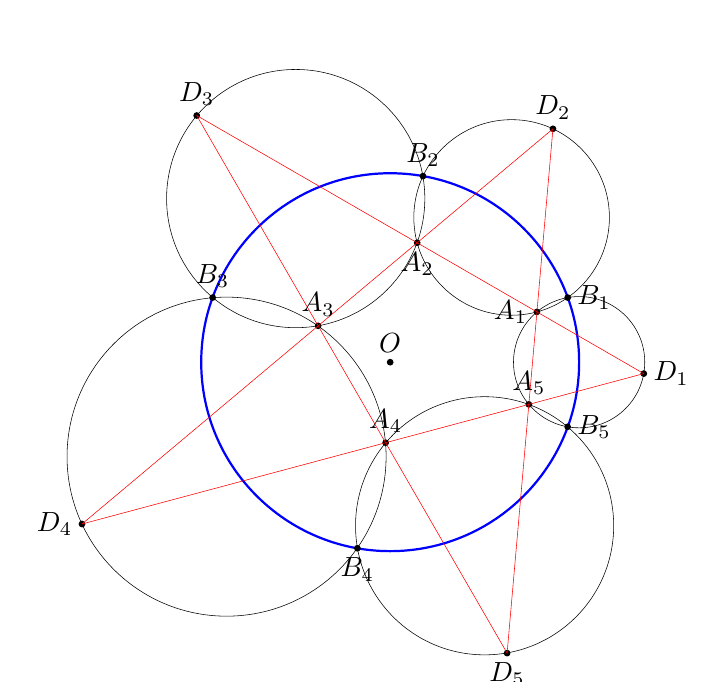
\begin{tikzpicture}[scale=1.2]
            \tkzDefPoints{0/0/O, 2/0/C_1}
            \tkzDefPointBy[rotation=center O angle 50](C_1) \tkzGetPoint{C_2}
            \tkzDefPointBy[rotation=center O angle 70](C_2) \tkzGetPoint{C_3}
            \tkzDefPointBy[rotation=center O angle 90](C_3) \tkzGetPoint{C_4}
            \tkzDefPointBy[rotation=center O angle 90](C_4) \tkzGetPoint{C_5}
            \tkzDefPointBy[rotation=center O angle 20](C_1) \tkzGetPoint{B_1}
            \tkzDefPointBy[rotation=center O angle 30](C_2) \tkzGetPoint{B_2}
            \tkzDefPointBy[rotation=center O angle 40](C_3) \tkzGetPoint{B_3}
            \tkzDefPointBy[rotation=center O angle 50](C_4) \tkzGetPoint{B_4}
            \tkzDefPointBy[rotation=center O angle 40](C_5) \tkzGetPoint{B_5}
            \tkzDrawCircle[blue, thick](O,C_1)
            \tkzDrawCircle[black](C_1,B_1)
            \tkzDrawCircle[black](C_2,B_2)
            \tkzDrawCircle[black](C_3,B_3)
            \tkzDrawCircle[black](C_4,B_4)
            \tkzDrawCircle[black](C_5,B_5)
            \tkzInterCC[common=B_1](C_1,B_1)(C_2,B_2) \tkzGetFirstPoint{A_1}
            \tkzInterCC[common=B_2](C_2,B_2)(C_3,B_3) \tkzGetFirstPoint{A_2}
            \tkzInterCC[common=B_3](C_3,B_3)(C_4,B_4) \tkzGetFirstPoint{A_3}
            \tkzInterCC[common=B_4](C_4,B_4)(C_5,B_5) \tkzGetFirstPoint{A_4}
            \tkzInterCC[common=B_5](C_5,B_5)(C_1,B_1) \tkzGetFirstPoint{A_5}
            \tkzInterLL(A_1,A_2)(A_5,A_4) \tkzGetPoint{D_1}
            \tkzInterLL(A_2,A_3)(A_1,A_5) \tkzGetPoint{D_2}
            \tkzInterLL(A_3,A_4)(A_2,A_1) \tkzGetPoint{D_3}
            \tkzInterLL(A_4,A_5)(A_3,A_2) \tkzGetPoint{D_4}
            \tkzInterLL(A_5,A_1)(A_4,A_3) \tkzGetPoint{D_5}
            \tkzDrawPoints[fill=black](O,B_1,B_2,B_3,B_4,B_5,A_1,A_2,A_3,A_4,A_5,D_1,D_2,D_3,D_4,D_5)
            \tkzDrawSegments[red](D_1,D_3 D_3,D_5 D_5,D_2 D_2,D_4 D_4,D_1)
            \tkzLabelPoints[above](O,B_2,B_3,A_3,A_4,A_5,D_2,D_3)
            \tkzLabelPoints[below](B_4,A_2,D_5)
            \tkzLabelPoints[right](B_1,B_5,D_1)
            \tkzLabelPoints[left](A_1,D_4)
        \end{tikzpicture}
    \end{figure}
\end{mybox}
\iftoggle{showanswer}{
\begin{mybox}[證明]{4em}{1em}{0.5em}
    原命題等價於以下的命題一
    $$
        \measuredangle{B_1B_2B_3}=\measuredangle{B_1B_4B_3}=\measuredangle{B_1B_5B_3}
    $$
    分解$\measuredangle{B_1B_2B_3}$
    $$
        \measuredangle{B_1B_2B_3}=\measuredangle{B_1B_2A_2}+\measuredangle{A_2B_2B_3}
    $$
    一方面
    $$
        \measuredangle{B_1B_2A_2}=\measuredangle{B_1A_1A_2}=\measuredangle{B_1A_1D_1}=\measuredangle{B_1B_5D_1}
    $$
    另一方面
    $$    
        \measuredangle{A_2B_2B_3}=\measuredangle{A_2A_3B_3}=\measuredangle{D_4A_3B_3}=\measuredangle{D_4B_4B_3}
    $$
    所以$\measuredangle{B_1B_2B_3}$可分解成
    $$
        \measuredangle{B_1B_2B_3}=\measuredangle{B_1B_5D_1}+\measuredangle{D_4B_4B_3}
    $$
    分別代入至命題一中，可以發現等價於以下的命題二
    $$
        \begin{cases}
            \measuredangle{B_1A_5D_4}=\measuredangle{B_1B_5D_1}\\
            \measuredangle{D_1A_4B_3}=\measuredangle{D_4B_4B_3}
        \end{cases}
    $$
    進一步利用四點共圓知識可知
    $$
        \begin{cases}
            \measuredangle{B_1B_5D_1}=\measuredangle{B_1A_5D_1}=\measuredangle{B_1A_5D_4}\\
            \measuredangle{D_4B_4B_3}=\measuredangle{D_4A_4B_3}=\measuredangle{D_1A_4B_3}
        \end{cases}
    $$
    所以命題二等價轉換至下面的命題三
    $$
        \begin{cases}
            \measuredangle{B_1B_4D_4}=\measuredangle{B_1A_5D_4}\\
            \measuredangle{D_1B_5B_3}=\measuredangle{D_1A_4B_3}
        \end{cases}
    $$
    即$B_1$、$B_4$、$A_5$、$D_4$四點共圓且$B_3$、$B_5$、$A_4$、$D_1$四點共圓。

    由上方的推導可知
    $$
        \measuredangle{B_1A_5D_4}=\measuredangle{B_1B_5D_1}=\measuredangle{B_1B_2A_2}=\measuredangle{B_1D_2A_2}=\measuredangle{B_1D_2D_4}
    $$
    及
    $$
        \measuredangle{D_1A_4B_3}=\measuredangle{D_4B_4B_3}=\measuredangle{A_2B_2B_3}=\measuredangle{A_2D_3B_3}=\measuredangle{D_1D_3B_3}
    $$
    所以$B_1$、$D_2$、$A_5$、$D_4$四點共圓且$B_3$、$D_3$、$A_4$、$D_1$四點共圓。

    因此命題三等價於以下的命題四
    \begin{quotation}
        \centering
        $B_4$、$D_2$、$A_5$、$D_4$四點共圓且$B_5$、$D_3$、$A_4$、$D_1$四點共圓。
    \end{quotation}
    利用 Angle Chasing 可直接得
    $$
        \measuredangle{D_2D_4B_4}=\measuredangle{A_3D_4B_4}=\measuredangle{A_3A_4B_4}=\measuredangle{D_5A_4B_4}=\measuredangle{D_5A_5B_4}=\measuredangle{D_2A_5B_4}
    $$
    及
    $$
        \measuredangle{D_3D_1B_5}=\measuredangle{A_1D_1B_5}=\measuredangle{A_1A_5B_5}=\measuredangle{D_5A_5B_5}=\measuredangle{D_5A_4B_5}=\measuredangle{D_3A_4B_5}
    $$
    由上方兩式可證得命題四成立，原命題得證。
\end{mybox}
}{}
\begin{mybox}[Problem 3]{6.5em}{1em}{0.5em}
    圓$\Gamma$上存在按照逆時針排列的十點$C_1$、$B_1$、$C_2$、$B_2$、$C_3$、$B_3$、$C_4$、$B_4$、$C_5$和$B_5$。
    
    記$B_0=B_5$，對於任意$i\in\left\{1,2,3,4,5\right\}$，都有$C_iB_i=C_iB_{i-1}=r_i$。
    
    記$\Omega_6=\Omega_1$，對於任意$i\in\left\{1,2,3,4,5\right\}$，設$\Omega_i$是以$C_i$為圓心且半徑為$r_i$的圓。
    圓$\Omega_i$和$\Omega_{i+1}$相交於兩個相異點，記不在$\Gamma$上的交點為$A_i$。

    記$A_6=A_1$、$A_0=A_5$和$A_{-1}=A_4$，對於任意$i\in\left\{1,2,3,4,5\right\}$，設直線$A_iA_{i+1}$與$A_{i-1}A_{i-2}$的交點為$D_i$。

    求證：對於任意$i\in\left\{1,2,3,4,5\right\}$，$D_i$都在圓$\Omega_i$上。
    \begin{figure}[H]
        \centering
        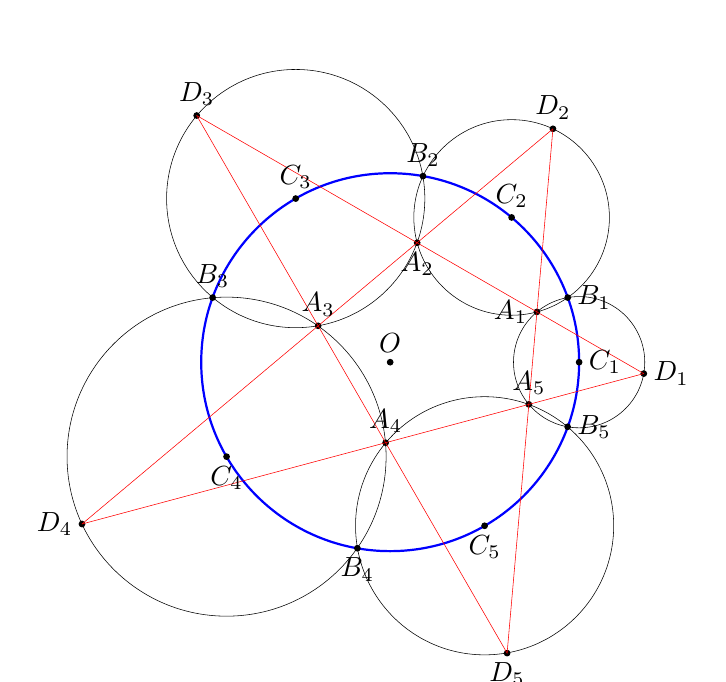
\begin{tikzpicture}[scale=1.2]
            \tkzDefPoints{0/0/O, 2/0/C_1}
            \tkzDefPointBy[rotation=center O angle 50](C_1) \tkzGetPoint{C_2}
            \tkzDefPointBy[rotation=center O angle 70](C_2) \tkzGetPoint{C_3}
            \tkzDefPointBy[rotation=center O angle 90](C_3) \tkzGetPoint{C_4}
            \tkzDefPointBy[rotation=center O angle 90](C_4) \tkzGetPoint{C_5}
            \tkzDefPointBy[rotation=center O angle 20](C_1) \tkzGetPoint{B_1}
            \tkzDefPointBy[rotation=center O angle 30](C_2) \tkzGetPoint{B_2}
            \tkzDefPointBy[rotation=center O angle 40](C_3) \tkzGetPoint{B_3}
            \tkzDefPointBy[rotation=center O angle 50](C_4) \tkzGetPoint{B_4}
            \tkzDefPointBy[rotation=center O angle 40](C_5) \tkzGetPoint{B_5}
            \tkzDrawCircle[blue, thick](O,C_1)
            \tkzDrawCircle[black](C_1,B_1)
            \tkzDrawCircle[black](C_2,B_2)
            \tkzDrawCircle[black](C_3,B_3)
            \tkzDrawCircle[black](C_4,B_4)
            \tkzDrawCircle[black](C_5,B_5)
            \tkzInterCC[common=B_1](C_1,B_1)(C_2,B_2) \tkzGetFirstPoint{A_1}
            \tkzInterCC[common=B_2](C_2,B_2)(C_3,B_3) \tkzGetFirstPoint{A_2}
            \tkzInterCC[common=B_3](C_3,B_3)(C_4,B_4) \tkzGetFirstPoint{A_3}
            \tkzInterCC[common=B_4](C_4,B_4)(C_5,B_5) \tkzGetFirstPoint{A_4}
            \tkzInterCC[common=B_5](C_5,B_5)(C_1,B_1) \tkzGetFirstPoint{A_5}
            \tkzInterLL(A_1,A_2)(A_5,A_4) \tkzGetPoint{D_1}
            \tkzInterLL(A_2,A_3)(A_1,A_5) \tkzGetPoint{D_2}
            \tkzInterLL(A_3,A_4)(A_2,A_1) \tkzGetPoint{D_3}
            \tkzInterLL(A_4,A_5)(A_3,A_2) \tkzGetPoint{D_4}
            \tkzInterLL(A_5,A_1)(A_4,A_3) \tkzGetPoint{D_5}
            \tkzDrawPoints[fill=black](O,C_1,C_2,C_3,C_4,C_5,B_1,B_2,B_3,B_4,B_5,A_1,A_2,A_3,A_4,A_5,D_1,D_2,D_3,D_4,D_5)
            \tkzDrawSegments[red](D_1,D_3 D_3,D_5 D_5,D_2 D_2,D_4 D_4,D_1)
            \tkzLabelPoints[above](O,C_2,C_3,B_2,B_3,A_3,A_4,A_5,D_2,D_3)
            \tkzLabelPoints[below](C_4,C_5,B_4,A_2,D_5)
            \tkzLabelPoints[right](C_1,B_1,B_5,D_1)
            \tkzLabelPoints[left](A_1,D_4)
        \end{tikzpicture}
    \end{figure}
\end{mybox}
\iftoggle{showanswer}{
\begin{mybox}[證明]{4em}{1em}{0.5em}
    為了方便討論，直接採用循環序號：
    \begin{quotation}
        \centering
        對於整數$i$、$j$，$\left(A_i,B_i,C_i,\Omega_i\right)=\left(A_j,B_j,C_j,\Omega_j\right)$當且僅當$5\left|i-j\right.$。
    \end{quotation}
    原命題等價於以下的命題一：
    $$
        \measuredangle{A_iD_iA_{i-1}}=\measuredangle{A_iB_iA_{i-1}}
    $$
    命題一可經過以下的推演，等價變換成下方的命題二：
    \begin{align*}
        &\measuredangle{A_iD_iA_{i-1}}=\measuredangle{A_iB_iA_{i-1}}\\
        \Leftrightarrow\quad&\measuredangle{\left(A_{i+1}A_i, A_{i-1}A_{i-2}\right)}=\measuredangle{\left(A_iB_i, A_{i-1}B_i\right)}\\
        \Leftrightarrow\quad&\measuredangle{\left(A_{i+1}A_i, A_iB_i\right)}+\measuredangle{\left(A_{i-1}B_{i-1}, A_{i-1}A_{i-2}\right)}
        =\measuredangle{\left(A_iB_i, A_{i-1}B_i\right)}-\measuredangle{\left(A_iB_i, A_{i-1}B_{i-1}\right)}\\
        \Leftrightarrow\quad&\measuredangle{A_{i+1}A_iB_i}+\measuredangle{B_{i-1}A_{i-1}A_{i-2}}=\measuredangle{B_{i-1}A_{i-1}B_i}
    \end{align*}
    在圓$\Omega_{i+1}$、$\Omega_i$和$\Omega_{i-1}$中分別有
    \begin{align*}
        &\measuredangle{A_{i+1}A_iB_i}=\measuredangle{A_{i+1}B_{i+1}B_i},\\
        &\measuredangle{B_{i-1}A_{i-1}A_{i-2}}=\measuredangle{B_{i-1}B_{i-2}A_{i-2}},\\
        &\measuredangle{B_{i-1}A_{i-1}B_i}=\frac{1}{2}\measuredangle{\overrightarrow{B_{i-1}C_iB_i}}
    \end{align*}
    所以命題二可以等價於以下的命題三：
    \begin{align*}
        &\measuredangle{A_{i+1}B_{i+1}B_i}+\measuredangle{B_{i-1}B_{i-2}A_{i-2}}=\frac{1}{2}\measuredangle{\overrightarrow{B_{i-1}C_iB_i}}\\
        \Leftrightarrow\quad&\measuredangle{\left(A_{i+1}B_{i+1}, B_{i+1}B_i\right)}+\measuredangle{\left(B_{i-1}B_{i-2},B_{i-2}A_{i-2}\right)}=\frac{1}{2}\measuredangle{\overrightarrow{B_{i-1}C_iB_i}}
    \end{align*}
    對於任意$j\in\mathbb{Z}$，$A_jB_j$都是圓$\Omega_j$和$\Omega_{j+1}$的根軸，所以有$C_jC_{j+1}\perp A_jB_j$。

    所以命題三可經過以下的推演，等價變換成下方的命題四：
    \begin{align*}
        &\measuredangle{\left(A_{i+1}B_{i+1}, B_{i+1}B_i\right)}+\measuredangle{\left(B_{i-1}B_{i-2},B_{i-2}A_{i-2}\right)}
        =\frac{1}{2}\measuredangle{\overrightarrow{B_{i-1}C_iB_i}}\\
        \Leftrightarrow\quad&\measuredangle{\left(A_{i+1}B_{i+1}, C_{i+1}C_{i+2}\right)}+\measuredangle{\left(C_{i+1}C_{i+2}, B_{i+1}B_i\right)}\\
        &+\measuredangle{\left(B_{i-1}B_{i-2},C_{i-2}C_{i-1}\right)}+\measuredangle{\left(C_{i-2}C_{i-1},B_{i-2}A_{i-2}\right)}
        =\frac{1}{2}\measuredangle{\overrightarrow{B_{i-1}C_iB_i}}\\
        \Leftrightarrow\quad&90^{\circ}+\measuredangle{\left(C_{i+1}C_{i+2}, B_{i+1}B_i\right)}+\measuredangle{\left(B_{i-1}B_{i-2},C_{i-2}C_{i-1}\right)}+90^{\circ}
        =\frac{1}{2}\measuredangle{\overrightarrow{B_{i-1}C_iB_i}}\\
        \Leftrightarrow\quad&\measuredangle{\left(C_{i+1}C_{i+2}, B_{i+1}B_i\right)}+\measuredangle{\left(B_{i-1}B_{i-2},C_{i-2}C_{i-1}\right)}
        =\frac{1}{2}\measuredangle{\overrightarrow{B_{i-1}C_iB_i}}\\
        \Leftrightarrow\quad&\measuredangle{\left(C_{i+1}C_{i+2}, B_{i+1}B_i\right)}+\measuredangle{\left(B_{i-1}B_{i-2},C_{i-2}C_{i-1}\right)}
        =\frac{1}{2}\measuredangle{\overrightarrow{B_{i-1}C_iB_i}}\\
        \Leftrightarrow\quad&\measuredangle{\left(C_{i+1}C_{i+2}, B_{i+1}C_{i+1}\right)}+\measuredangle{\left(B_{i+1}C_{i+1}, B_{i+1}B_i\right)}\\
        &+\measuredangle{\left(B_{i-1}B_{i-2},C_{i-1}B_{i-2}\right)}+\measuredangle{\left(C_{i-1}B_{i-2},C_{i-2}C_{i-1}\right)}
        =\frac{1}{2}\measuredangle{\overrightarrow{B_{i-1}C_iB_i}}\\
        \Leftrightarrow\quad&\measuredangle{C_{i+2}C_{i+1}B_{i+1}}+\measuredangle{C_{i+1}B_{i+1}B_i}+\measuredangle{B_{i-1}B_{i-2}C_{i-1}}+\measuredangle{B_{i-2}C_{i-1}C_{i-2}}
        =\frac{1}{2}\measuredangle{\overrightarrow{B_{i-1}C_iB_i}}
    \end{align*}
    在圓$\Gamma$上有
    \begin{align*}
        &\measuredangle{C_{i+2}C_{i+1}B_{i+1}}=\measuredangle{C_{i+2}C_iB_{i+1}}\\
        &\measuredangle{C_{i+1}B_{i+1}B_i}=\measuredangle{C_{i+1}C_iB_i}\\
        &\measuredangle{B_{i-1}B_{i-2}C_{i-1}}=\measuredangle{B_{i-1}C_iC_{i-1}}\\
        &\measuredangle{B_{i-2}C_{i-1}C_{i-2}}=\measuredangle{B_{i-2}C_iC_{i-2}}
    \end{align*}
    所以命題四等價於以下的命題五：
    $$
        \measuredangle{C_{i+2}C_iB_{i+1}}+\measuredangle{C_{i+1}C_iB_i}+\measuredangle{B_{i-1}C_iC_{i-1}}+\measuredangle{B_{i-2}C_iC_{i-2}}
        =\frac{1}{2}\measuredangle{\overrightarrow{B_{i-1}C_iB_i}}
    $$
    對於任意$j\in\mathbb{Z}$，$B_{j-1}$、$C_j$、$B_{j+1}$在圓$\Gamma$上按逆時針排列。
    對於$k\in\mathbb{Z}$且$5\nmid{k-j}$，$C_k$和$C_j$必然分別在$B_{j-1}B_j$的兩側。
    結合$C_jB_j=C_jB_{j-1}$，配合圓周角定理可知 $C_kC_j$為$\angle{B_{j-1}C_kB_j}$ 的內角平分線。因此有
    $$
        \frac{1}{2}\measuredangle{\overrightarrow{B_{j-1}C_kB_j}}=\measuredangle{B_{j-1}C_kC_j}=\measuredangle{C_jC_kB_j}
    $$
    利用這個結論可以得出
    \begin{align*}
        &\measuredangle{C_{i+2}C_iB_{i+1}}=\frac{1}{2}\measuredangle{\overrightarrow{B_{i+2}C_iB_{i+1}}}\\
        &\measuredangle{C_{i+1}C_iB_i}=\frac{1}{2}\measuredangle{\overrightarrow{B_{i+1}C_iB_i}}\\
        &\measuredangle{B_{i-1}C_iC_{i-1}}=\frac{1}{2}\measuredangle\overrightarrow{{B_{i-1}C_iB_{i-2}}}\\
        &\measuredangle{B_{i-2}C_iC_{i-2}}=\frac{1}{2}\measuredangle{\overrightarrow{B_{i-2}C_iB_{i-3}}}
    \end{align*}
    所以命題五可經過以下的推演，等價變換成下方的命題六：
    \begin{align*}
        &\measuredangle{C_{i+2}C_iB_{i+1}}+\measuredangle{C_{i+1}C_iB_i}+\measuredangle{B_{i-1}C_iC_{i-1}}+\measuredangle{B_{i-2}C_iC_{i-2}}
        =\frac{1}{2}\measuredangle{\overrightarrow{B_{i-1}C_iB_i}}\\
        \Leftrightarrow\quad&\frac{1}{2}\measuredangle{\overrightarrow{B_{i+2}C_iB_{i+1}}}+\frac{1}{2}\measuredangle{\overrightarrow{B_{i+1}C_iB_i}}
        +\frac{1}{2}\measuredangle\overrightarrow{{B_{i-1}C_iB_{i-2}}}+\frac{1}{2}\measuredangle{\overrightarrow{B_{i-2}C_iB_{i-3}}}
        =\frac{1}{2}\measuredangle{\overrightarrow{B_{i-1}C_iB_i}}\\
        \Leftrightarrow\quad&\frac{1}{2}\measuredangle{\overrightarrow{B_{i+2}C_iB_i}}+\frac{1}{2}\measuredangle\overrightarrow{{B_{i-1}C_iB_{i-3}}}
        =\frac{1}{2}\measuredangle{\overrightarrow{B_{i-1}C_iB_i}}
    \end{align*}
    利用循環序號可知$B_{i-3}=B_{i+2}$，所以必有
    \begin{align*}
        \frac{1}{2}\measuredangle{\overrightarrow{B_{i+2}C_iB_i}}+\frac{1}{2}\measuredangle\overrightarrow{{B_{i-1}C_iB_{i-3}}}
        &=\frac{1}{2}\measuredangle{\overrightarrow{B_{i+2}C_iB_i}}+\frac{1}{2}\measuredangle\overrightarrow{{B_{i-1}C_iB_{i+2}}}\\
        &=\frac{1}{2}\left(\measuredangle\overrightarrow{{B_{i-1}C_iB_{i+2}}}+\measuredangle{\overrightarrow{B_{i+2}C_iB_i}}\right)\\
        &=\frac{1}{2}\measuredangle{\overrightarrow{B_{i-1}C_iB_i}}
    \end{align*}
    由此可知命題六成立，即原命題得證。
\end{mybox}
}{}
\begin{mybox}[Problem 4]{6.5em}{1em}{0.5em}
    設圓$\Gamma_1$與$\Gamma_2$相交於$D$和$P$兩點，圓$\Gamma_2$與$\Gamma_3$相交於$E$和$P$兩點，圓$\Gamma_3$與$\Gamma_1$相交於$F$和$P$兩點。
    在$\Gamma_2$上任取一點$C\notin\left\{D,E,P\right\}$，設$CD$交圓$\Gamma_1$於另一點$B\neq D$，$CE$交圓$\Gamma_3$於另一點$A\neq E$。

    求證：$A$、$F$、$B$三點共線。
    此定理稱為「密克定理的逆定理」。
\end{mybox}
\iftoggle{showanswer}{
\begin{mybox}[證明]{4em}{1em}{0.5em}
    原命題等價於以下的命題一
    $$
        \measuredangle{PFA}=\measuredangle{PFB}
    $$
    因為$A$、$E$、$F$、$P$四點共圓$\Gamma_3$，所以有$\measuredangle{PFA}=\measuredangle{PEA}$。

    因為$B$、$F$、$D$、$P$四點共圓$\Gamma_1$，所以有$\measuredangle{PFB}=\measuredangle{PDB}$。

    所以命題一等價於以下的命題二
    $$
        \measuredangle{PEA}=\measuredangle{PDB}
    $$
    因為$C$、$E$、$A$三點共線，所以有$\measuredangle{PEA}=\measuredangle{PEC}$。

    因為$B$、$D$、$C$三點共線，所以有$\measuredangle{PDB}=\measuredangle{PDC}$。

    所以命題二可以等價於以下的命題三
    $$
        \measuredangle{PEC}=\measuredangle{PDC}
    $$
    因為$C$、$D$、$E$、$P$四點共圓$\Gamma_2$，所以有$\measuredangle{PEC}=\measuredangle{PDC}$，命題二成立，原命題得證。
\end{mybox}
}{}
\begin{mybox}[Problem 5]{6.5em}{1em}{0.5em}
    在$\triangle{ABC}$中，$D$、$E$、$F$分別為直線$BC$、$CA$、$AB$上的點，且$\left\{D,E,F\right\}\cap\left\{A,B,C\right\}=\emptyset$。
    記$\triangle{AEF}$、$\triangle{BFD}$和$\triangle{CDE}$的外接圓分別為$\Omega_1$、$\Omega_2$和$\Omega_3$。
    直線$AD$分別與$\Omega_1$、$\Omega_2$和$\Omega_3$交於$X$、$Y$和$Z$點，其中$X\neq A$且$D\notin\left\{Y,Z\right\}$。

    求證：$YX/XZ=BD/DC$。
\end{mybox}
\iftoggle{showanswer}{
\begin{mybox}[證明]{4em}{1em}{0.5em}
    由密克定理知$\Omega_1$、$\Omega_2$和$\Omega_3$三圓交於一點$K$。利用無向分角定理可知
    \begin{align*}
        \frac{YX}{XZ}&=\frac{KY}{KZ}\cdot\frac{\sqrt{1-\cos{2\measuredangle{YKX}}}}{\sqrt{1-\cos{2\measuredangle{XKZ}}}}\\
        \frac{BD}{DC}&=\frac{KB}{KC}\cdot\frac{\sqrt{1-\cos{2\measuredangle{BKD}}}}{\sqrt{1-\cos{2\measuredangle{DKC}}}}
    \end{align*}
    利用 Angle Chasing 可知
    \begin{align*}
        \measuredangle{YKX}&=\measuredangle{YKF}+\measuredangle{FKX}=\measuredangle{YDF}+\measuredangle{FAX}\\
        &=\measuredangle{ADF}+\measuredangle{FAD}=\measuredangle{AFD}\\
        &=\measuredangle{BFD}=\measuredangle{BKD}
    \end{align*}
    \begin{align*}
        \measuredangle{XKZ}&=\measuredangle{XKE}+\measuredangle{EKZ}=\measuredangle{XAE}+\measuredangle{EDZ}\\
        &=\measuredangle{DAE}+\measuredangle{EDA}=\measuredangle{DEA}\\
        &=\measuredangle{DEC}=\measuredangle{DKC}
    \end{align*}
    所以原命題等價於
    $$
        \frac{KY}{KZ}=\frac{KB}{KC}
    $$
    再次利用 Angle Chasing 可知
    $$
        \begin{cases}
            \measuredangle{BKY}=\measuredangle{BDY}=\measuredangle{CDZ}=\measuredangle{CKZ}\\
            \measuredangle{KYB}=\measuredangle{KDB}=\measuredangle{KDC}=\measuredangle{KZC}
        \end{cases}    
    $$
    由此可知 $\triangle{BKY}$ 與 $\triangle{CKZ}$ 旋轉相似，即有
    $$
        \frac{KB}{KC}=\frac{KY}{KZ}
    $$
    原命題得證。
\end{mybox}
}{}
\end{document}